%%%%%%%%%%%%%%%%%%%%%%%%%%%%%%%%%%%%%%%%%
% Jacobs Landscape Poster
% LaTeX Template
% Version 1.1 (14/06/14)
%
% Created by:
% Computational Physics and Biophysics Group, Jacobs University
% https://teamwork.jacobs-university.de:8443/confluence/display/CoPandBiG/LaTeX+Poster
% 
% Further modified by:
% Nathaniel Johnston (nathaniel@njohnston.ca)
%
% This template has been downloaded from:
% http://www.LaTeXTemplates.com
%
% License:
% CC BY-NC-SA 3.0 (http://creativecommons.org/licenses/by-nc-sa/3.0/)
%
%%%%%%%%%%%%%%%%%%%%%%%%%%%%%%%%%%%%%%%%%

%----------------------------------------------------------------------------------------
%	PACKAGES AND OTHER DOCUMENT CONFIGURATIONS
%----------------------------------------------------------------------------------------

\documentclass[final]{beamer}

\usepackage[scale=1.24]{beamerposter} % Use the beamerposter package for laying out the poster

\usetheme{confposter} % Use the confposter theme supplied with this template

\setbeamercolor{block title}{fg=ngreen,bg=white} % Colors of the block titles
\setbeamercolor{block body}{fg=black,bg=white} % Colors of the body of blocks
\setbeamercolor{block alerted title}{fg=white,bg=dblue!70} % Colors of the highlighted block titles
\setbeamercolor{block alerted body}{fg=black,bg=dblue!10} % Colors of the body of highlighted blocks
% Many more colors are available for use in beamerthemeconfposter.sty

%-----------------------------------------------------------
% Define the column widths and overall poster size
% To set effective sepwid, onecolwid and twocolwid values, first choose how many columns you want and how much separation you want between columns
% In this template, the separation width chosen is 0.024 of the paper width and a 4-column layout
% onecolwid should therefore be (1-(# of columns+1)*sepwid)/# of columns e.g. (1-(4+1)*0.024)/4 = 0.22
% Set twocolwid to be (2*onecolwid)+sepwid = 0.464
% Set threecolwid to be (3*onecolwid)+2*sepwid = 0.708

\newlength{\sepwid}
\newlength{\onecolwide}
\newlength{\twocolwide}
\newlength{\threecolwide}
\setlength{\paperwidth}{48in} % A0 width: 46.8in
\setlength{\paperheight}{36in} % A0 height: 33.1in
\setlength{\sepwid}{0.024\paperwidth} % Separation width (white space) between columns
\setlength{\onecolwide}{0.22\paperwidth} % Width of one column
\setlength{\twocolwide}{0.464\paperwidth} % Width of two columns
\setlength{\threecolwide}{0.708\paperwidth} % Width of three columns
\setlength{\topmargin}{-0.5in} % Reduce the top margin size
%-----------------------------------------------------------

\usepackage{graphicx}  % Required for including images

\usepackage{booktabs} % Top and bottom rules for tables

%----------------------------------------------------------------------------------------
%	TITLE SECTION 
%----------------------------------------------------------------------------------------

\title{Pixel Telescope to test pixel Phase II ROCs and sensors} % Poster title

\author{Caleb Fangmeier} % Author(s)

\institute{Dept.\ of Physics and Astronomy, Univ.\ of Nebraska \-- Lincoln} % Institution(s)

%----------------------------------------------------------------------------------------

\begin{document}

\addtobeamertemplate{block end}{}{\vspace*{2ex}} % White space under blocks
\addtobeamertemplate{block alerted end}{}{\vspace*{2ex}} % White space under highlighted (alert) blocks

\setlength{\belowcaptionskip}{2ex} % White space under figures
\setlength\belowdisplayshortskip{2ex} % White space under equations

\begin{frame}[t] % The whole poster is enclosed in one beamer frame


\begin{column}{\sepwid}\end{column} % Empty spacer column

\begin{columns}[t]
\begin{column}{\paperwidth}

  \begin{figure}
    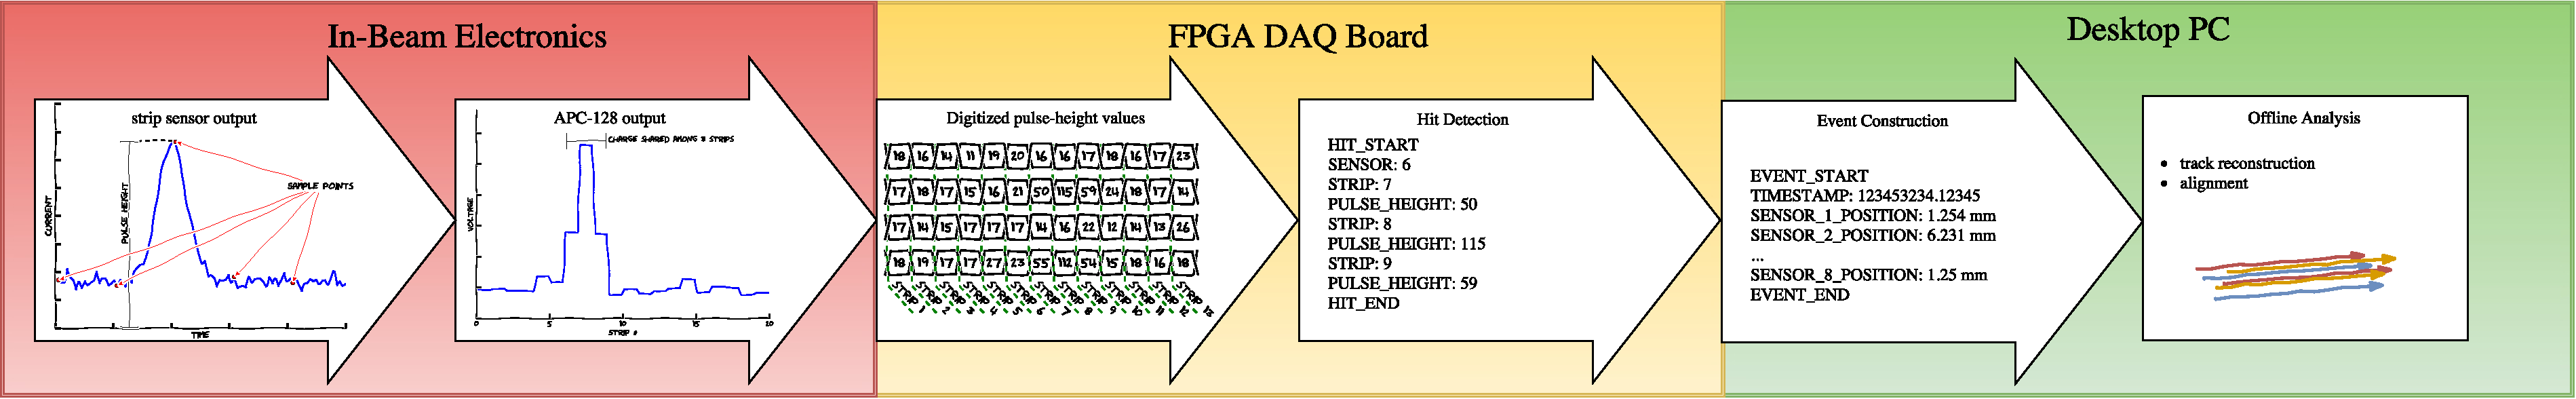
\includegraphics[width=0.98\textwidth]{figures/Telescope_Data_Flow}
  \end{figure}

\end{column}
\end{columns}

% \vspace{2in}
\begin{columns}[t]
\begin{column}{\onecolwide}
  \begin{itemize}
    \item ahd asdf s fpasoidfksajdAIDS asdihf wfasdfASHDf y8238rjdsf saJDFASIDF asd fhasdfoua hdsfaSDFJ HIE hi dfsadhifoa hdsoifhasdF asdhifa shdifohsad
    \item ahd asdf s fpasoidfksajdAIDS asdihf wfasdfASHDf y8238rjdsf saJDFASIDF asd fhasdfoua hdsfaSDFJ HIE hi dfsadhifoa hdsoifhasdF asdhifa shdifohsad
    \item ahd asdf s fpasoidfksajdAIDS asdihf wfasdfASHDf y8238rjdsf saJDFASIDF asd fhasdfoua hdsfaSDFJ HIE hi dfsadhifoa hdsoifhasdF asdhifa shdifohsad
    \item ahd asdf s fpasoidfksajdAIDS asdihf wfasdfASHDf y8238rjdsf saJDFASIDF asd fhasdfoua hdsfaSDFJ HIE hi dfsadhifoa hdsoifhasdF asdhifa shdifohsad
  \end{itemize}
\end{column}
\begin{column}{\onecolwide}
  \begin{itemize}
    \item ahd asdf s fpasoidfksajdAIDS asdihf wfasdfASHDf y8238rjdsf saJDFASIDF asd fhasdfoua hdsfaSDFJ HIE hi dfsadhifoa hdsoifhasdF asdhifa shdifohsad
    \item ahd asdf s fpasoidfksajdAIDS asdihf wfasdfASHDf y8238rjdsf saJDFASIDF asd fhasdfoua hdsfaSDFJ HIE hi dfsadhifoa hdsoifhasdF asdhifa shdifohsad
    \item ahd asdf s fpasoidfksajdAIDS asdihf wfasdfASHDf y8238rjdsf saJDFASIDF asd fhasdfoua hdsfaSDFJ HIE hi dfsadhifoa hdsoifhasdF asdhifa shdifohsad
    \item ahd asdf s fpasoidfksajdAIDS asdihf wfasdfASHDf y8238rjdsf saJDFASIDF asd fhasdfoua hdsfaSDFJ HIE hi dfsadhifoa hdsoifhasdF asdhifa shdifohsad
  \end{itemize}
\end{column}
\begin{column}{\onecolwide}
  \begin{itemize}
    \item ahd asdf s fpasoidfksajdAIDS asdihf wfasdfASHDf y8238rjdsf saJDFASIDF asd fhasdfoua hdsfaSDFJ HIE hi dfsadhifoa hdsoifhasdF asdhifa shdifohsad
    \item ahd asdf s fpasoidfksajdAIDS asdihf wfasdfASHDf y8238rjdsf saJDFASIDF asd fhasdfoua hdsfaSDFJ HIE hi dfsadhifoa hdsoifhasdF asdhifa shdifohsad
    \item ahd asdf s fpasoidfksajdAIDS asdihf wfasdfASHDf y8238rjdsf saJDFASIDF asd fhasdfoua hdsfaSDFJ HIE hi dfsadhifoa hdsoifhasdF asdhifa shdifohsad
    \item ahd asdf s fpasoidfksajdAIDS asdihf wfasdfASHDf y8238rjdsf saJDFASIDF asd fhasdfoua hdsfaSDFJ HIE hi dfsadhifoa hdsoifhasdF asdhifa shdifohsad
  \end{itemize}
\end{column}
\end{columns} % End of all the columns in the poster
\vspace{5mm}
\hrule


\end{frame} % End of the enclosing frame

\end{document}

